\documentclass[
	a4paper,
	oneside,
	BCOR = 10mm,
	DIV = 12,
	12pt,
	headings = normal,
]{scrartcl}

%%% Length calculations
\usepackage{calc}
%%%

%%% Support for color
\usepackage{xcolor}
\definecolor{lightblue}{HTML}{03A9F4}
\definecolor{red}{HTML}{F44336}
%%%

%%% Including graphics
\usepackage{graphicx}
%%%

%%% Font selection
\usepackage{fontspec}

\setromanfont{STIX Two Text}[
	SmallCapsFeatures = {LetterSpace = 8},
]

\setsansfont{IBM Plex Sans}[
	Scale = MatchUppercase,
]

\setmonofont{IBM Plex Mono}[
	Scale = MatchUppercase,
]
%%%

%%% Math typesetting
\usepackage{amsmath}

\usepackage{unicode-math}
\setmathfont{STIX Two Math}

\usepackage{IEEEtrantools}
%%%

%%% List settings
\usepackage{enumitem}
\setlist[enumerate]{%
	label*      = {\arabic*.},
	leftmargin  = *,
	labelindent = \parindent,
	topsep      = 1\baselineskip,
	parsep      = 0\baselineskip,
	itemsep     = 1\baselineskip,
	noitemsep, % override itemsep
}

\setlist[itemize]{%
	label*      = {—},
	leftmargin  = *,
	labelindent = \parindent,
	topsep      = 1\baselineskip,
	parsep      = 0\baselineskip,
	itemsep     = 1\baselineskip,
	noitemsep, % override itemsep
}

\setlist[description]{%
	font        = {\rmfamily\upshape\bfseries},
	topsep      = 1\baselineskip,
	parsep      = 0\baselineskip,
	itemsep     = 0\baselineskip,
}

%%%

%%% Structural elements typesetting
\setkomafont{pagenumber}{\rmfamily\upshape}
\setkomafont{disposition}{\rmfamily\bfseries}

% Sectioning
\RedeclareSectionCommand[
	beforeskip = -1\baselineskip,
	afterskip  = 1\baselineskip,
	font       = {\normalsize\bfseries\scshape},
]{section}

\RedeclareSectionCommand[
	beforeskip = -1\baselineskip,
	afterskip  = 1\baselineskip,
	font       = {\normalsize\bfseries\itshape},
]{subsection}

\RedeclareSectionCommand[
	beforeskip = -1\baselineskip,
	afterskip  = 1\baselineskip,
	font       = {\normalsize\bfseries},
]{subsubsection}

\RedeclareSectionCommand[
	beforeskip = -1\baselineskip,
	afterskip  = -0.5em,
	font       = {\normalsize\mdseries\scshape\addfontfeatures{Letters = {UppercaseSmallCaps}}},
]{paragraph}
%%%

%%% Typographic enhancements
\usepackage{microtype}
%%%

%%% Language-specific settings
\usepackage{polyglossia}
\setmainlanguage{ukrainian}
\setotherlanguages{english}
%%%

%%% Captions
\usepackage{caption}
\usepackage{subcaption}

%\DeclareCaptionLabelFormat{closing}{#2)}
%\captionsetup[subtable]{labelformat = closing}

%\captionsetup[subfigure]{labelformat = closing}

\captionsetup[table]{%
	aboveskip = 0\baselineskip,
	belowskip = 0\baselineskip,
}

\captionsetup[figure]{%
	aboveskip = 1\baselineskip,
	belowskip = 0\baselineskip,
}

\captionsetup[subfigure]{%
	labelformat = simple,
	labelformat = brace,
}
%%%

%%% Hyphenated ragged typesetting
\usepackage{ragged2e}
%%%

%%% Table typesetting
\usepackage{booktabs}
\usepackage{longtable}

\usepackage{multirow}

\usepackage{array}
\newcolumntype{v}[1]{>{\RaggedRight\arraybackslash\hspace{0pt}}p{#1}}
\newcolumntype{b}[1]{>{\Centering\arraybackslash\hspace{0pt}}p{#1}}
\newcolumntype{n}[1]{>{\RaggedLeft\arraybackslash\hspace{0pt}}p{#1}}
%%%

%%% Drawing
\usepackage{tikz}
\usepackage{tikzscale}
\usetikzlibrary{arrows.meta} % Stealth arrow tips
\usetikzlibrary{positioning}
\usetikzlibrary{shapes.geometric} % Stealth arrow tips
%%%

%%% SI units typesetting
\usepackage{siunitx}
\sisetup{%
	output-decimal-marker = {,},
	exponent-product      = {\cdot},
	inter-unit-product    = \ensuremath{{} \cdot {}},
	per-mode              = symbol,
}
%%%

%%% Framing code listings
\usepackage{tcolorbox}
\tcbuselibrary{breakable}
\tcbuselibrary{minted}
\tcbuselibrary{skins}

\newtcblisting[
	auto counter,
	list inside,
	number within = section,
]{listingpython}[3][]{%
	minted language = python,
	minted style    = bw,
	minted options  = {%
		linenos,
		tabsize = 4,
		breaklines,
		% breakanywhere,
		fontsize = \footnotesize,
		autogobble
	},
	%
	% empty,
	sharp corners,
	colframe         = black,
	colback          = black!0,
	leftrule         = 0em,
	rightrule        = 0em,
	toprule          = 1pt, % orig = 0pt
	bottomrule       = 1pt, % orig = 0pt
	titlerule        = 0.5pt,
	colbacktitle     = black!0,
	coltitle         = black,
	toptitle         = 0.3em,
	bottomtitle      = 0.1em,
	borderline north = {1pt}{0pt}{black},
	borderline south = {1pt}{0pt}{black},
	before skip      = \intextsep,
	after  skip      = \intextsep,
	title            = {Лістинг \thetcbcounter: #2},
	list entry       = {\protect\numberline{\thetcbcounter}#2},
	left = 0em,
	right = 0em,
	%
	listing only,
	breakable,
	%
	label = {#3},
	%
	#1
}

\newtcbinputlisting[auto counter, list inside, number within = section]{\inputpython}[4][]{%
	minted language = python,
	minted style    = bw,
	minted options  = {%
		linenos,
		tabsize = 4,
		breaklines,
		breakbytokenanywhere,
		fontsize = \footnotesize,
	},
	%
	% empty,
	sharp corners,
	colframe         = black,
	colback          = black!0,
	leftrule         = 0em,
	rightrule        = 0em,
	toprule          = 0pt, % orig = 0pt
	bottomrule       = 0pt, % orig = 0pt
	titlerule        = 0.5pt,
	colbacktitle     = black!0,
	coltitle         = black,
	toptitle         = 0.3em,
	bottomtitle      = 0.1em,
	borderline north = {1pt}{0pt}{black},
	borderline south = {1pt}{0pt}{black},
	before skip      = \intextsep,
	after  skip      = \intextsep,
	title            = {Лістинг \thetcbcounter: #3},
	list entry       = {\protect\numberline{\thetcbcounter}#3},
	left = 0em,
	right = 0em,
	%
	listing file={#2},
	listing only,
	breakable,
	%
	label = {#4},
	%
	#1
}

% Customize minted
\usepackage{minted}
\setmintedinline{%
	style = bw,
	breaklines,
}

% Customize minted line numbers
\renewcommand{\theFancyVerbLine}{\ttfamily\scriptsize\arabic{FancyVerbLine}}

%%%

%%% Sideways table
\usepackage{pdflscape}
%%%

%%% Wrap text after sideways table
\usepackage{afterpage}
%%%

%%% Links and hyperreferences
\usepackage{hyperref}
\hypersetup{%
	bookmarksnumbered = true,
	colorlinks      = false,
	linkbordercolor = red,
	urlbordercolor  = lightblue,
	pdfborderstyle  = {/S/U/W 1.5},
}
%%%

%%% Length adjustments
% Set baselineskip, default is 14.5 pt
\linespread{1.068966} % ~15.5 pt
\setlength{\emergencystretch}{1em}
\setlength{\parindent}{1.5em}
\newlength{\gridunitwidth}
\setlength{\gridunitwidth}{\textwidth / 12}
%%%

%%% Custom commands
\newcommand{\allcaps}[1]{{\addfontfeatures{LetterSpace = 8, Kerning = Off}#1}}
\newcommand{\filename}[1]{\texttt{#1}}
\newcommand{\progname}[1]{\texttt{#1}}
\newcommand{\modulename}[1]{\texttt{#1}}
%%%

%%% Custom math commands
\newcommand{\longvar}[1]{\mathit{#1}}
\newcommand{\sdiv}{\mathbin{/}}
%%%

\begin{document}

\begin{titlepage}
		\begin{center}
			Міністерство освіти і~науки України\\
			Національний авіаційний університет\\
			Навчально-науковий інститут комп'\-ютерних інформаційних технологій\\
			Кафедра комп'\-ютеризованих систем управління

			\vspace{\fill}
				Лабораторна робота №5\\
				з~дисципліни «Комп'\-ютерні системи»\\
				на~тему «Архітектура конвеєрних обчислювальних систем»\\
				Варіант~№3

			\vspace{\fill}

			\begin{flushright}
				Виконав:\\
				студент \allcaps{ННІКІТ}\\
				групи СП-325\\
				Клокун В.\,Д.\\
				Перевірив:\\
				Ковальов М.\,О.
			\end{flushright}

			Київ 2019
		\end{center}
	\end{titlepage}

	\section{Мета роботи}
		Аналіз структур конвеєрних обчислювальних систем.

	\section{Загальні теоретичні відомості}
		Конвеєр являє собою процесор, розділений на~$P$ частин (шарів, рядків), виконуючих послідовно етапи кожної обчислювальної задачі (операції). В~той час як~$j$-й~шар процесора виконує $j$-й~етап деякої $k$-ї~задачі, $(j-1)$-й~шар може виконувати $(j-1)$-й~етап $(k+1)$-ї~задачі, $(j-2)$-й~шар може виконувати $(j-2)$-й~етап $(k+2)$-ї~задачі і~так далі, тобто 1-й~шар може у~цей же~час виконувати 1-й~етап $(i+j-1)$-ї~задачі, де~$j = 2, \dots, P$. Таким чином, кожна задача або операція виконується за~$P$ етапів при проходженні усіх $P$ шарів конвеєрного процесора.

		В~обчислювальних системах (ОС) з~конвеєрним процесором може виконуватися одночасно декілька ($P$) операцій по~перетворенню даних, що~відповідає визначенню обчислюваної системі. Проте ці~операції в~будь-який момент часу обов’язково знаходяться на~різних етапах виконання й~у~принципі не~можуть починатися всі одночасно.

		Конвеєрні системи з~роздільним керуванням, орієнтовані на~паралелізм незалежних гілок (тип~К1). На~рис.~\ref{fig:mpp-t01} зображена конвеєрна система з~роздільним керуванням. Вона складається з~$P$ пристроїв керування (ПК)~— по~кількості шарів, на~які розділений конвеєрний процесор. Принципово важливим є~наявність $P$ роздільних вузлів формування адреси наступної інструкції. Можливо, що~в~кожного ПК~є~свої індексні та~базові регістри, регістри ключів захисту та~інші індивідуальні ланцюги. Частина ланцюгів може бути загальної для різних ПК~(наприклад, формувач адреси операндів, дешифратор коду операцій), які використовуються усіма ПК~по~черзі. Ці~загальні ланцюги на~рисунку включені до~складу шарів процесора.

		\begin{figure}[!htbp]
			\centering
			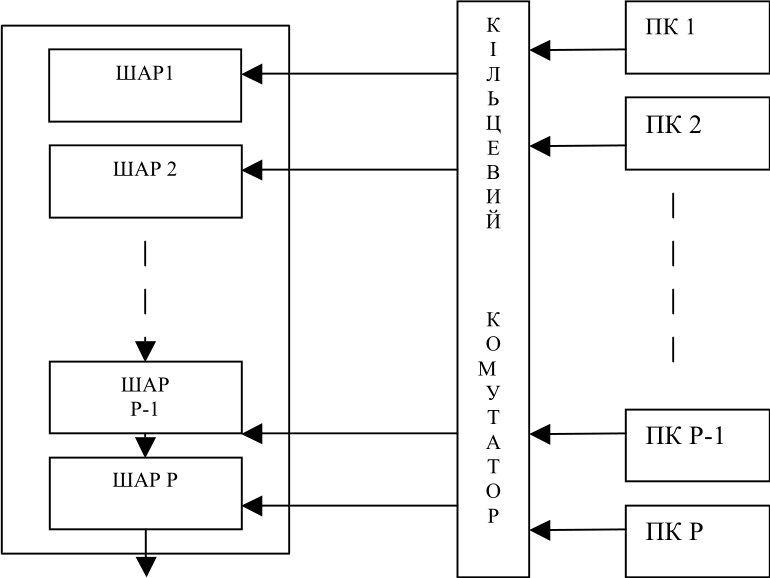
\includegraphics[height=9\baselineskip]{./assets/y03s02-compsys-lab-05-p01-mpp-t01.jpg}
			\caption{}
			\label{fig:mpp-t01}
		\end{figure}

		Пристрій керування приєднаний до~шарів конвеєрного процесора через кільцевий комутатор. Комутатор улаштований так, що~в~1-му~такті роботи ОС~до~1-го~шару процесора підключено 1-й~ПК, який починає виконувати свої задачі (операції); в~2-му~такті 1-й~ПК~переключається на~2-й~шар процесора, а~до~1-го~шару підключається 2-й~ПК~і~т.д. У~р-му~такті 1-й~ПК~підключено до~$P$-го~шару процесора, де~завершується виконання 1-ї~задачі (операції), до~$(P-1)$-го~шару підключається 2-й~ПК,..., до~1-го~шару підключено $P$-й~ПК. Після закінчення 1-ї~задачі (операції) 1-й~ПК~в~$(p+1)$-му~такті 1-й~пристрій знову підключається до~1-го~шару процесора, де~починається виконання 2-ї~задачі (операції) і~т.д.

		Система, побудована зазначеним чином, аналогічна за~своїми можливостями $P$-процесорній системі типу~М1 (з~роздільним керуванням) і~орієнтована на~використання паралелізму незалежних гілок.

		Розглянутий конвеєрний процесор є~багатофункціональним, тобто дозволяє виконувати одночасно різні операції. Проте при цьому тривалість такту роботи шарів процесора залежить від виконуваних операцій та~буде визначатися часом виконання самої тривалої операції.

		Конвеєрні системи з~загальним керуванням, орієнтовані на~використання паралелізму суміжних операцій. Пристрій керування (рис.~\ref{fig:mpp-t02}) один, але регістрів для збереження інструкцій (РгІ) стільки ж, скільки шарів є~в~процесорі. Інструкція~1 програми зчитується в~РгІ(1), та~в~1-му~шарі процесора починається виконання. В~наступному такті інструкція~1 передається в~РгІ(2), її~виконання продовжує 2-й~шар процесора, а~до~РгІ(1) зчитується інструкція~2 програми та~в~1-му~шарі конвеєрного процесора починається її~виконання і~т.\,д.

		\begin{figure}[!htbp]
			\centering
			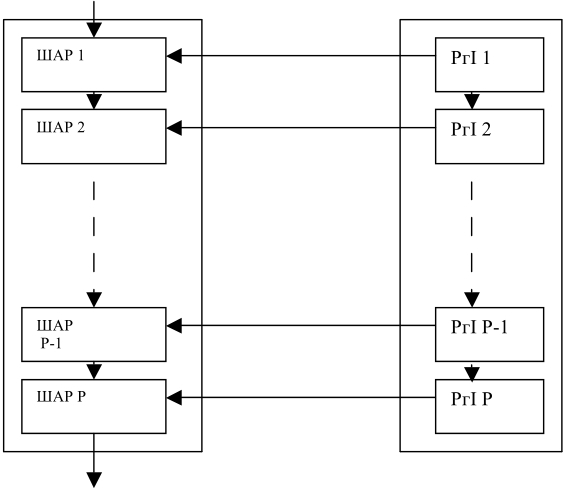
\includegraphics[height=14\baselineskip]{./assets/y03s02-compsys-lab-05-p01-mpp-t02.jpg}
			\caption{}
			\label{fig:mpp-t02}
		\end{figure}

		Конвеєрна система, побудована зазначеним чином, аналогічна багатопроцесорній системі М2 (із~загальним керуванням). Будемо називати її~ОС~типу~К2.

		Розглянутий конвеєрний процесор системи типу~К2 теж є~багатофункціональним. Будемо розрізняти динамічну та~статичну перебудови процесора для виконання різних операцій.

		Динамічна перебудова конвеєра (тип~К2.1) дозволяє виконувати різні операції одночасно в~різних шарах конвеєра. Але так само, як~і~для систем типу~К1, такт конвеєра в~кожний момент часу буде визначатися часом виконання самої тривалої операції (у~випадку використання конвеєра зі~змінним тактом) або часом виконання самої тривалої з~усіх операцій, на~виконання якої орієнтовано даний багатофункціональний конвеєр (у~випадку використання конвеєра з~постійним тактом).

		У~випадку статичної перебудови конвеєра (тип~К2.2) на~виконання нової операції необхідно дочекатися звільнення конвеєра від попередньої операції та~тільки після цього завантажувати наступну операцію (якщо вона відрізняється від виконуваної).

		У~випадку конвеєра з~постійним тактом його тривалість дорівнює часу виконання найтривалішої операції, яка в~принципі може бути виконана багатофункціональним конвеєром.

	\section{Хід роботи}
		Вихідними даними для виконання лабораторної роботи за~варіантом №~3 є~арифметичний вираз~\eqref{eq:expr}.
		\begin{IEEEeqnarray}{rCl}
			\label{eq:expr}
			(A + B \sdiv C \times G) \times (K + E + L) \sdiv R + D.
		\end{IEEEeqnarray}
		За~даним виразом складаємо його дерево~— граф потоків обчислень~(рис.~\ref{fig:expression-tree}).

		\begin{figure}[!htbp]
			\centering
			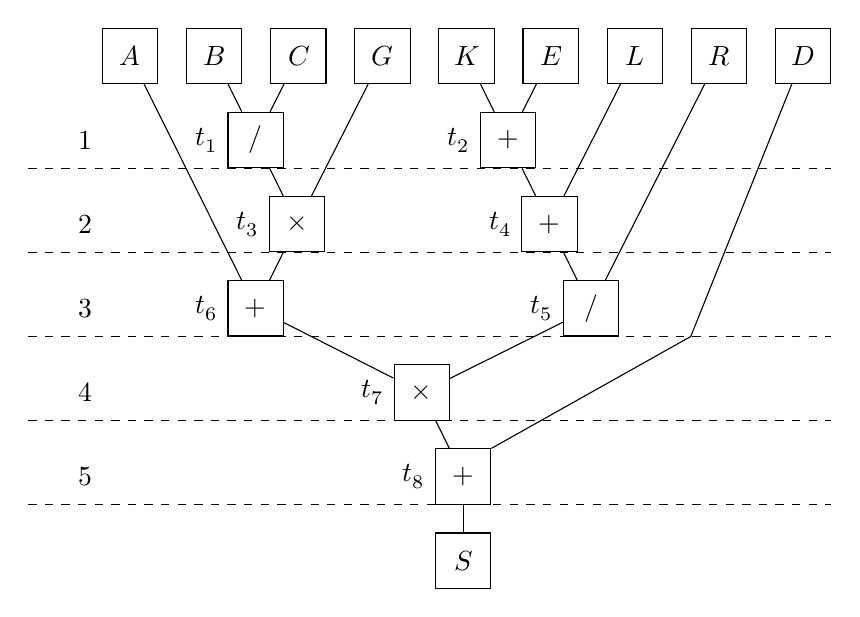
\begin{tikzpicture}[]
				\tikzset{main node/.style={draw,minimum size=2em}}
				\tikzset{every label/.style={label position=left}}
				\begin{scope}
					\node[main node] (l05-a) {$A$};
					\node[main node, right = 1em of l05-a] (l05-b) {$B$};
					\node[main node, right = 1em of l05-b] (l05-c) {$C$};
					\node[main node, right = 1em of l05-c] (l05-g) {$G$};
					\node[main node, right = 1em of l05-g] (l05-k) {$K$};
					\node[main node, right = 1em of l05-k] (l05-e) {$E$};
					\node[main node, right = 1em of l05-e] (l05-l) {$L$};
					\node[main node, right = 1em of l05-l] (l05-r) {$R$};
					\node[main node, right = 1em of l05-r] (l05-d) {$D$};
				\end{scope}

				\begin{scope}[every node/.style = {anchor=north west}]
					% Level 01
					\node[main node, label={$t_1$}, below right = 1em and 1.50em of l05-b.south west]  (l04-div-01) {$\sdiv$};
					\node[main node, label={$t_2$}, below right = 1em and 1.50em of l05-k.south west]  (l04-add-01) {$+$};

					% Level 02
					\node[main node, label={$t_3$}, below right = 1em and 1.50em of l04-div-01.south west]  (l03-mul-01) {$\times$};
					\node[main node, label={$t_4$}, below right = 1em and 1.50em of l04-add-01.south west]  (l03-add-01) {$+$};

					% Level 03
					\node[main node, label={$t_6$}, below left  = 1em and 1.50em of l03-mul-01.south east] (l02-add-01) {$+$};
					\node[main node, label={$t_5$}, below right = 1em and 1.50em of l03-add-01.south west] (l02-div-01) {$\sdiv$};

					% Level 04
					\node[main node, label={$t_7$}, below right = 1em and 6.00em of l02-add-01.south west] (l01-mul-01) {$\times$};

					% Level 05
					\node[main node, label={$t_8$}, below right = 1em and 1.50em of l01-mul-01.south west] (root-plus) {$+$};

					% Root
					\node[main node, below = 1em of root-plus] (root-S) {$S$};
				\end{scope}

				\begin{scope}
					\path[draw]
					(root-S)     edge node {} (root-plus)
					% Make intermediate point at horizontal intersection of t_5 and D
					(root-plus.north east)  -- (l02-div-01.south -| l05-r.south west) -- (l05-d)
					(root-plus)  edge node {} (l01-mul-01)
					(l01-mul-01) edge node {} (l02-add-01)
					             edge node {} (l02-div-01)
					(l02-add-01) edge node {} (l05-a)
					             edge node {} (l03-mul-01)
					(l02-div-01) edge node {} (l03-add-01)
					             edge node {} (l05-r)
					(l03-mul-01) edge node {} (l04-div-01)
					             edge node {} (l05-g)
					(l03-add-01) edge node {} (l04-add-01)
					             edge node {} (l05-l)
					(l04-div-01) edge node {} (l05-b)
					             edge node {} (l05-c)
					(l04-add-01) edge node {} (l05-k)
					             edge node {} (l05-e)
					;
				\end{scope}

				\begin{scope}
				%\path[dashed] (current bounding box.west) -- (current bounding box.east);
						\node [minimum size = 2em, anchor = north east, below left = 1em and 0em of l05-a.south west] (l05) {Ярус 1};
						\node [minimum size = 2em, below = 1em of l05.south] (l04) {Ярус 2};
						\node [minimum size = 2em, below = 1em of l04.south] (l03) {Ярус 3};
						\node [minimum size = 2em, below = 1em of l03.south] (l02) {Ярус 4};
						\node [minimum size = 2em, below = 1em of l02.south] (l01) {Ярус 5};

						\draw [dashed] (l05.south west) -- (l05.south west -| l05-d.east);
						\draw [dashed] (l04.south west) -- (l04.south west -| l05-d.east);
						\draw [dashed] (l03.south west) -- (l03.south west -| l05-d.east);
						\draw [dashed] (l02.south west) -- (l02.south west -| l05-d.east);
						\draw [dashed] (l01.south west) -- (l01.south west -| l05-d.east);
				\end{scope}

			\end{tikzpicture}
			\caption{Дерево арифметичного виразу $(A + B \sdiv C \times G) \times (K + E + L) \sdiv R + D$}
			\label{fig:expression-tree}
		\end{figure}

	\section{Висновок}
		Виконуючи дану лабораторну роботу, ми~проаналізували структури конвеєрних обчислювальних систем.

\end{document}

